\section{Обзор на разгледаните метрики}
В тази глава ще представим основните свойства на разгледаните от нас метрики. Като споменахме вече, ще се фокусираме върху пространства, описващи компактни обекти които \emph{не} притежават хоризонти на събитията. Можем допълнително да класифицираме разглежданите метрики като такива, които притежават физическа сингулярност (най-общо наричани голи сингулярности), и напълно регулярни.
 
\subsection{Пространствено-времеви тунели}
За обща дефиниция на пространствено времеви тунел можем да приемем следното (CIТE VISSER HERE):\\

\emph{Всеки компактен регион от пространство-времето, който притежава топологично проста граница, но топологично нетривиален обем.}\\\newline
Тълкуването на тази дефиниция е следната: Подобно пространство-време притежава свойството да "свързва"$\,$ два отдалечени (потенциално причинно откъснати) региона. Топологино простата граница в горната дефиниция тогава изразява факта, че тези структури са локализирани така, че самото пространство-време е асиамптотически плоско. Топологично нетривиалният обем изразява факта, че за да се "свържат"$\,$ два далечни региона, пространството \emph{трябва} да е неедносвързано. Подобни структури за пръв път са били обсъдени в литературата скоро след откриването на решението на Шварцшилд$^1$. Тези първоначални разглеждания са описвали т.н. \emph{непроходими тунели} и затова са предизвикали особен теоретичен интерес. Едва с появата на влиятелната публикация на Морис и Торн CITE MORIS AND THORNE HERE, описваща сферично симетрични \emph{проходими тунели}, тези обекти стават релевантни в теоретичната астрофизика.\\

Описването на проходими тунели представлява до голяма степен "обратна задача"$\,$ на решаването на уравненията на Айнщайн-Хилбърт. Започва се с постулат на желаните от обекта свойства и анзац за метриката, удовлетворяващ тези свойства, след което той се замества в полевите уравнения за да се установи типът материя, нужен за поддържане на обекта. Анзацът, който ще използваме e предложен от Тео CITE TEO HERE като обобщение на резултатите на CITE MORIS AND THORN HERE за \emph{въртящият се случай} е:
 \setlength{\footskip}{0pt}
\lfoot{\noindent\makebox[\linewidth]{\rule{\textwidth}{0.4pt}}
	\small$^1$ Още през 1916 г. Людвиг Флам CITE показва, че в решението на Шварцшилд може да се намери "втори регион"$\,$ (в последствие, с въвеждането на координати на Крускал, наречен бяла дупка), свързан със самата черна дупка чрез "мост". Тази идея е повдигната отново едва през 1935 г. от Айнщайн и Розен CITE, които преоткриват тази структура, и тя става известна като мост на Айнщайн-Розен. В последствие Фюлер и Уилър CITE показват, че този мост \emph{не} може да бъде прекосен. Може да се покаже, че тази структура е координатен (при това динамичен!) артефакт - за по-подробна дискусия насочваме читателя към CITE HERE.}
	
\begin{equation}
	ds^2 = -N^2(r,\theta)dt^2 + \frac{dr^2}{1 - \frac{b(r,\theta)}{r}} + r^2K^2(r,\theta)\left[d\theta^2 + \sin^2\theta\left(d\phi + \omega(r,\theta)dt\right)^2\right].
\end{equation}
Функциите $N(r,\theta)$ и $\omega(r,\theta)$ са добре известни от 3+1 формулировката на ОТО като функция на времевия поток (lapse function) и на отместването (shift function), докато $b(r,\theta)$ е специфична за тунелите и се нарича функция на формата. Следвайки CITE MORIS AND THORNE HERE, най-общите изисквания към проходим тунел са:\\

\textbf{1) Липса на хоризонт на събитията.} Метричният анзац (5.1), бивайки аксиално симетричен, притежава вектор на Килинг от вида $k^\mu = \delta_t^\mu + \omega_0\delta^\mu_\phi$, където $\omega_0 = -\frac{g_{t\phi}}{g_{\phi\phi}}^1$. В този случай можем да дефинираме еднозначно хоризонт на събитията като повърхнина, върху която е изпълнено условието $k_\mu k^\mu = 0$. Тогава изискването за липса на хоризонт на събитията е еквивалентно на:

\begin{equation}
g_{\mu\nu} (\delta_t^\mu + \omega_0\delta^\mu_\phi) (\delta_t^\nu + \omega_0\delta^\nu_\phi) \ne 0 \rightarrow g_{tt} - \frac{g_{t\phi}^2}{g_{\phi\phi}} \ne 0.
\end{equation}\newline
Ако презапишем анзацът (5.1) чрез компонентите $g_{\mu\nu}$ виждаме, че тя има вида:
\begin{equation}
	ds^2 = \left(g_{tt} - \frac{g_{t\phi}^2}{g_{\phi\phi}}\right)dt + g_{rr}dr^2 + g_{\theta\theta}d\theta^2 + g_{\phi\phi}\left(d\phi + \frac{g_{t\phi}}{g_{\phi\phi}}d\phi\right)^2.
\end{equation}
Това ни показва, че условието (5.2) е еквивалентно на $N(r,\theta)\ne 0\quad \forall r\in\mathcal{D}_r,\,\forall \theta\in[0,\pi]$, където $\mathcal{D}_r$ е дефиниционното множество на радиалната координата, което ще бъде коментирано в условие 3). За да запази пространството (5.3) своята Лоренцова сигнатура обаче, ние ще наложим условието $N(r,\theta) > 0$. Тогава е удобно да представим $N(r,\theta)$ като:
\begin{equation}
	N(r,\theta) \equiv e^{\Phi(r,\theta)}, \quad |\Phi(r,\theta)| < \infty,\,\, \forall r\in\mathcal{D}_r,\,\,\forall\theta\in[0,\pi]
\end{equation}
\textbf{2) Асимптотическа плоскост.} Това условие идва от общото физическо съображение, че всеки компактен обект, представляващ локално сгъстяване на материя, не бива да упражнява гравитационно влияние на безкрайност. Това налага следните условия върху метричните функции:

\begin{equation}
	\begin{aligned}
		&N(r,\theta) \xrightarrow[r\rightarrow\infty]{} 1 - \frac{A}{r},\quad \frac{b(r,\theta)}{r} \xrightarrow[r\rightarrow\infty]{} \frac{B}{r} \\
		&\omega(r,\theta)\xrightarrow[r\rightarrow\infty]{} \frac{C}{r^3}\quad\qquad  K(r,\theta) \xrightarrow[r\rightarrow\infty]{} 1,
	\end{aligned}
\end{equation}
където $A$, $B$ и $C$ са константи.
\lfoot{\noindent\makebox[\linewidth]{\rule{\textwidth}{0.4pt}}
	\small$^1$ Величината $\omega_0$ представлява ъгловата скорост на т.н. \emph{локално невъртящ се наблюдател}. За него имаме, че моментът на импулса му $L_z$ e равен на 0. В аксиално-симетрични пространства от това следва:
	\begin{equation*}
		L_z = k_\phi = g_{\phi\phi}\frac{d\phi}{d\lambda} + g_{t\phi}\frac{dt}{d\lambda} = 0\rightarrow \frac{d\phi}{dt} = -\frac{g_{t\phi}}{g_{\phi\phi}} := \omega_0.
	\end{equation*}
	Ненулевата стойност на $\omega_0$ e проявление на т.н. \emph{eфект на увличане на инерциалните наблюдатели}, породен от смесеният член $g_{t\phi}$ (т.е. от въртенето на централният обект).}

\newpage

\textbf{3) Метриката притежава топологията на "тунел".} Това означава, че радиалната координата е ограничена отдолу до минималното разстояние $r_0(\theta)$ такова, че: $1 - \frac{b(r_0,\theta)}{r_0} \ge 0 ,\,\,\forall r\in \mathcal{D}_r = [r_0(\theta),\infty],\,\,\forall\theta\in[0,\pi]^{\,\,1}$. За да покажем защо това условие реализира топологията на "тунел"$,$ нека вложим сечението $t = \text{const},\,\,\theta = \text{const}$ на пространството (5.1) в $\mathcal{R}^3$. Линейният елемент тогава заема формата:
\begin{equation}
	ds^2 = \frac{dr^2}{1 - \frac{b(r,\theta)}{r}} + r^2K^2(r,\theta)\sin^2\theta d\phi^2 = \frac{d\rho^2}{1 - \frac{\beta(\rho,\theta)}{\rho}} + \rho^2(\theta)d\phi^2,
\end{equation}
където сме въвели новата координата $\rho = rK(r,\theta)\sin\theta$. Приравняваме (5.6) към линейният елемент на $\mathcal{R}^3$ в цилиндрични координати:
\begin{equation}
	ds^2_{\mathcal{R}^3} = d\rho^2 + \rho^2d\phi^2 + dz^2 = \left[1 + \left(\frac{dz}{d\rho}\right)^2\right]d\rho^2 + \rho^2d\phi^2.
\end{equation}
Идеята на това влагане е да използваме координатата $z$ за визуализиране на тунелната структура. Приравнявайки (5.6) и (5.7) получаваме следното уравнение:
\begin{equation}
	\frac{dz}{d\rho} = \pm \left(\frac{\rho}{\beta(\rho,\theta)} - 1\right)^{-1/2}.
\end{equation}
Кривата $z(\rho,\theta)$ се нарича \emph{функция на влагането}. Виждаме, че за да е реална функция е нужно да бъде изпълнено условието $\frac{\rho(r)}{\beta(\rho(r),\theta)}-1\ge 0$. Равенството дефинира т.н. \emph{гърловина} на тунела $r_0(\theta)$, която играе ролята на долната граница на радиалната координата, спомената по-горе.\\
За илюстрация нека решим уравнението на влагането (5.8) за $b(r,\theta) = \text{const} = b_0$ и $K(r,\theta) = 1$. Получаваме $z(r) = \pm 2b_0\sqrt{\frac{r}{b_0} - 1}$. Това решение е начертано на фигура \ref{WH_embedding}. Забелязваме, че разходимостта на (5.8) върху гърловината e нужна за формирането на "тунел"$\,$ между регионите, белязани като $I$ и $II$, зависещ от функционалната форма на $b(r)$. Именно от тука следва наименуването ѝ като "функция на формата". Съществуването на реални решения на (5.8) обаче, не е достатъчно да гарантира топология която свързва две далечни области. Нужно е да се наложи допълнително условие гласящо, че кривата, описвана от $z(\rho)$, трябва да се "отваря навън"$\,$ от гърловината (т.н. flare out condition). Математически това се изразява в изискването CITE TEO HERE:
\begin{equation}
	\frac{d^2\rho}{dz^2}\bigg\vert_{r = r_0(\theta)} > 0\rightarrow \frac{b(r,\theta) - r\partial_rb(r,\theta)}{2b^2(r,\theta)}\bigg\vert_{r = r_0(\theta)} > 0.
\end{equation}\newline
\lfoot{\noindent\makebox[\linewidth]{\rule{\textwidth}{0.4pt}}
	\small$^1$ Това ограничение върху минималната стойност на радиалната координата има за цел да запази Лоренцовата сигнатура на метриката в цялото пространство.}
Виждаме, че това условие е изпълнено за частният случай от фигура \ref{WH_embedding}.\\

\begin{minipage}{15em}
	\centering
	\hspace{-0.99cm}
	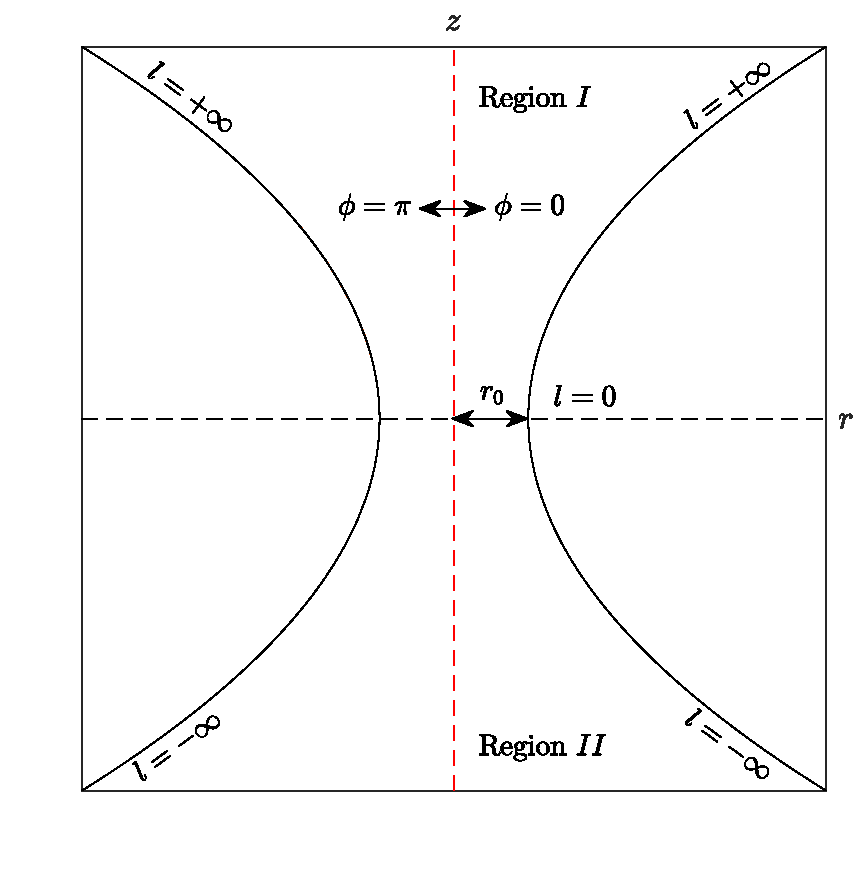
\includegraphics[scale = 0.4]{WH_embedding.pdf}
	\captionof{figure}[Влагаща диаграма на пространствено-времеви тунел]{\small Влагаща диаграма на пространствено-времеви тунел за частният случай на $b(r,\theta) = \text{const} = b_0$}
	\label{WH_embedding}
\end{minipage}
\begin{minipage}{16em}
	Можем да забележим обаче, линейният елемент (5.1) притежава сингулярност върху гърловината $r_0(\theta) = b(r_0,\theta)$. Подобно на координатната сингулярност в решението на Шварцшилд при $r = 2M$, тя може да бъде отстранена с подходяща смяна на координатите 
	\begin{equation}
	r	 \rightarrow \ell^2(r,\theta) = r^2 - b^2(r,\theta).
	\end{equation}
	
	Тогава разходящият член от (5.1) се превръща в:
	\begin{equation}
		\frac{dr^2}{1 - \frac{b(r,\theta)}{r}} \rightarrow \left[1 + \frac{b(r,\theta)}{r}\right]d\ell^2
	\end{equation}
	
\end{minipage}\\\newline
Координатата $\ell(r,\theta)$ се нарича \emph{глобална}, понеже позволява гладко преминаване през гърловината на тунела. Условно идентифицираме регионът с $\ell >0$ като "нашата"$\,$ страна на тунела, докато този с $\ell < 0$ като "другата"$\,$ страна.\\

\textbf{4) Липса на физически сингулярности.} Пресмятайки скалара на Ричи $R$, може да се покаже, че той има следната форма върху гърловината $r_0(\theta) = b(r_0,\theta)$ CITE HRE:
\begin{equation}
	\begin{aligned}
		(rK)^2R = &-\frac{3}{2}\frac{(\partial_\theta b)^2}{(r - b)^2} - \frac{\partial^2_\theta b}{r - b}
	- \frac{2}{r^2K^2}\left[\partial_\theta \Phi + \frac{\partial_\theta K}{K} + \frac{\partial_\theta b}{r}\right]\tan\theta + \\ 
	& + \text{reg. terms}.
	\end{aligned}
\end{equation}
Виждаме, че за избегнем сингулярности върху оста на въртене $\theta = 0,\pi$, e нужно да занулим следните членове върху гърловината:
\begin{equation}
	\partial_\theta \Phi(r_0(\theta),\theta) = 0\big\vert_{\theta = 0,\pi},\, \partial_\theta K(r_0(\theta),\theta)\big\vert_{\theta = 0,\pi} = 0,\,\partial_\theta b(r_0(\theta),\theta)\big\vert_{\theta = 0,\pi} = 0.
\end{equation}
Докато за да избегнем сингулярности върху самата гърловина е нужно да наложим:
\begin{equation}
	\partial_\theta b(r,\theta)\big\vert_{r = r_0} = 0,\, \partial^2_\theta b(r,\theta)\big\vert_{r = r_0} = 0.
\end{equation}
Отново можем да видим, че частният случай от фигура \ref{WH_embedding} изпълнява всички тези условия.\\

\lfoot{}
\textbf{Вече можем да запишем конкретната форма на анзацът (5.1) използван от нас:}
\begin{equation}
	N(r,\theta) = e^{-\frac{r_0}{r} - \alpha\frac{r_0^2}{r^2}},\, b(r,\theta) = r_0,\, K(r,\theta) = 1,\, \omega(r,\theta) = \frac{2a}{r^3}
\end{equation}
\newpage
\subsubsection{Физическа интерпретация на параметрите на тунела}

Понеже методиката за построяване на решение, описващо тунел в пространство-времето, не започва с постулирането на разпределение от материя, е нужно специално внимание за интерпретирането на параметрите в развитието (5.5).\\

\textbf{Интерпретация на константата $B$.} Нейната стойност зависи директно от асимптотичното поведение на функцията на формата и следователно няма обща физическа интерпретация сама по себе си (още повече след като имаме свободата да избираме природата на $b(r,\theta)$, стига тя да удовлетворява свойствата (5.13) и (5.14)). По-скоро на нея трябва да се гледа като условие върху тензора на момента и импулса, и следователно, върху материята която генерира тунела.\\

\textbf{Интерпретация на константата $A$.} Понеже разглежданият общ анзац (5.1) е статичен, можем да пресметнем за него интегралите на Комар. По-конкретно нека пресметнем \emph{масата на Комар} $M_{\text{Komar}}$. Тя се задава с израза:
\begin{equation}
	M_{\text{Komar}} = -\frac{1}{4\pi}\int_{\partial\Sigma}\nabla^\mu k^\nu_t dS_{\mu\nu} =  -\frac{1}{4\pi}\int_{\partial\Sigma}\nabla^\mu k^\nu_t\left[n_\mu\sigma_\nu - n_\nu\sigma_\mu\right] \sqrt{\sigma}d^2y,
\end{equation}
където $k^\mu_t = (-1,0,0,0)$ и интегралите са по границата на времеподобно 3-мерно многообразие $\Sigma_t$, дефинирано като $\mathcal{M} = \mathcal{R} \times \Sigma_t$. Т.е. $\Sigma_t$ представлява пространственото сечение на $\mathcal{M}$ за фиксирано координатно време $t$. Може да се покаже, че (5.15) не зависи от избора $\Sigma_t$, поради което индексът е изпуснат. Тогава можем да интерпретираме $\partial\Sigma$ като пространствена безкрайност $r\rightarrow\infty$ и $\sqrt{\sigma}$ като индуцирана метрика върху 2-мерната сфера $r = \text{const}, t = \text{const}$. Векторите $n_\mu = - (\sqrt{-g_{tt}}, 0, 0, 0)$ и $\sigma_\nu = (0, \sqrt{g_{rr}},0 ,0)$ представляват нормалите на $\Sigma$ и $\partial\Sigma$. Пресмятайки изразът (5.16), използвайки анзацът (5.15), получаваме следният резултат REF APENDIX HERE:
\begin{equation}
	M_{\text{Komarr}} = r_0 \xrightarrow[(5.15)]{} A = M_{\text{Komar}}
\end{equation}

\textbf{Интерпретация на константата $C$.} Нека сега пресметнем \emph{момента на импулса на Комар} $J_{\text{Komar}}$, дефиниран като:
\begin{equation}
	J_{\text{Komar}} = \frac{1}{8\pi}\int_{\partial\Sigma}\nabla^\mu k^\nu_\phi dS_{\mu\nu} = \frac{1}{8\pi}\int_{\partial\Sigma}\nabla^\mu k^\nu_\phi\left[n_\mu\sigma_\nu - n_\nu\sigma_\mu\right] \sqrt{\sigma}d^2y,
\end{equation}
където $k^\phi = (0, 0, 0, 1)$. Отново, самото изчисление може да се намери в REF APENDIX HERE, крайният резултат е следният:
\begin{equation}
	J_\text{Komar} = a\xrightarrow[(5.15)]{} C = 2J_\text{Komar}, 
\end{equation}
където $a$ представлява нормираният момент на импулса на тунела.
\subsubsection{Оптична проява - фотонни орбити и сенки}
Замествайки явната форма на метриката (5.1) в уравнението на Хамилтон-Якоби, и отчитайки чистата радиална зависимост на метричните функции (5.15), извършваме разделянето на променливите за да стигнем до следната система от динамични уравнения:
\begin{subequations}
	\begin{equation}
		\frac{dt}{d\lambda} = \frac{E - \omega(r)L_z}{N^2(r)}
	\end{equation}
	\begin{equation}
		\frac{N(r)}{\sqrt{1 - \frac{b(r)}{r}}}\frac{dr}{d\lambda} = \pm \sqrt{R(r)}
	\end{equation}
	\begin{equation}
		r^2K^2(r)\frac{d\theta}{d\lambda} = \pm \sqrt{\Theta(\theta)}
	\end{equation}
	\begin{equation}
		\frac{d\phi}{d\lambda} = \omega(r)\frac{E - \omega(r)L_z}{N^2(r)} + \frac{L_z}{r^2K^2(r)\sin^2\theta},
	\end{equation}
\end{subequations}
където потенциалите $R(r)$ и $\Theta(\theta)$ се задават от функциите:
\begin{subequations}
	\begin{equation}
		R(r) = -C\frac{N^2(r)}{r^2K^2(r)} + (E - \omega(r)L_z)^2 - m^2N^2(r)\\
	\end{equation}
	\begin{equation}
		\Theta(\theta) = C - \frac{L_z^2}{\sin^2\theta}
	\end{equation}
\end{subequations}
и $C = k_\theta^2 + \frac{L_z^2}{\sin^2\theta}$ е константата на Картер. Може да отбележим някой неща за тази система:\\\newline
1) Тя е валидна когато всички метрични функции в (5.1) имат само радиална зависимост. Това представлява по-общ случай, който обхваща и нашият конкретен избор на функции (5.15).\\\newline
2) Уравнение (5.20г) има интересното свойство, че по явен начин отделя ефекта на увличане на инициални наблюдатели (левият член) от "естествената"$\,$ азимутална динамика (десният член). Т.е то има вида $\frac{d\phi}{d\lambda} = g(a,r) + f(r),\,\, g(a = 0, r) = 0$\newpage

Както споменахме вече в глава 2, основен интерес за нас представляват фотонните орбити (поради директната им връзка с видимата форма на обектите на небето). Нека използваме системата (5.20) за да намерим условията, при които тези фотони попадат в \emph{нестабилни} кръгови орбити около тунела:
\begin{subequations}
	\begin{equation}
	\left(\frac{dr}{d\lambda}\right)^2 = \frac{1}{N^2(r)}\left(1 - \frac{b(r)}{r}\right)R(r) = - V_\text{eff} = 0
	\end{equation}
	\begin{equation}
		\frac{d^2r}{d\lambda^2} = -\frac{1}{2}\frac{dV_{\text{eff}}}{dr} = 0
	\end{equation}
	\begin{equation}
		\frac{d^2V_\text{eff}}{dr^2} \le 0
	\end{equation}
\end{subequations}

\newpage
\subsection{Голи сингуларности на Джанис-Нюман-Уиникър}
